%%%%%%%%%%%%%%%%%%%%%%%%%%%%%%%%%%%%%%%%%%%%%%%%%%%%%%%%%%%%%%%%%%%%%%%%%%%%%%%
%%%%%%%%%%%%%%%%%%%%%%%%%%%%%%%%%%%%%%%%%%%%%%%%%%%%%%%%%%%%%%%%%%%%%%%%%%%%%%%
%%
%%
%%             c.     R  E  S  O  U  R  C  E  S 
%%
%%
%%%%%%%%%%%%%%%%%%%%%%%%%%%%%%%%%%%%%%%%%%%%%%%%%%%%%%%%%%%%%%%%%%%%%%%%%%%%%%%
%%%%%%%%%%%%%%%%%%%%%%%%%%%%%%%%%%%%%%%%%%%%%%%%%%%%%%%%%%%%%%%%%%%%%%%%%%%%%%%
\section{Resources (inlcuding project costs)}
%\smallskip \smallskip \noindent
%Resources and timelines should entirely reflect the project and nothing else. Link the budget to the proposed activities as accurately as possible.
%Feasibility is key.\\
%Remember to use whole Euro integers only, when preparing the budget table.
%Make sure the numbers on the table match with the numbers on the A forms.
%Use this table as it is and don’t reformat it.
%Delete all the superscript numbers in final draft to get rid of the text in footer. You will most likely need the space for your justification.
%%
%\smallskip
%\smallskip
%\noindent
Here we summarize and justify the budget.

\begin{figure}
  \begin{center}
    \hspace{-0.5cm}
    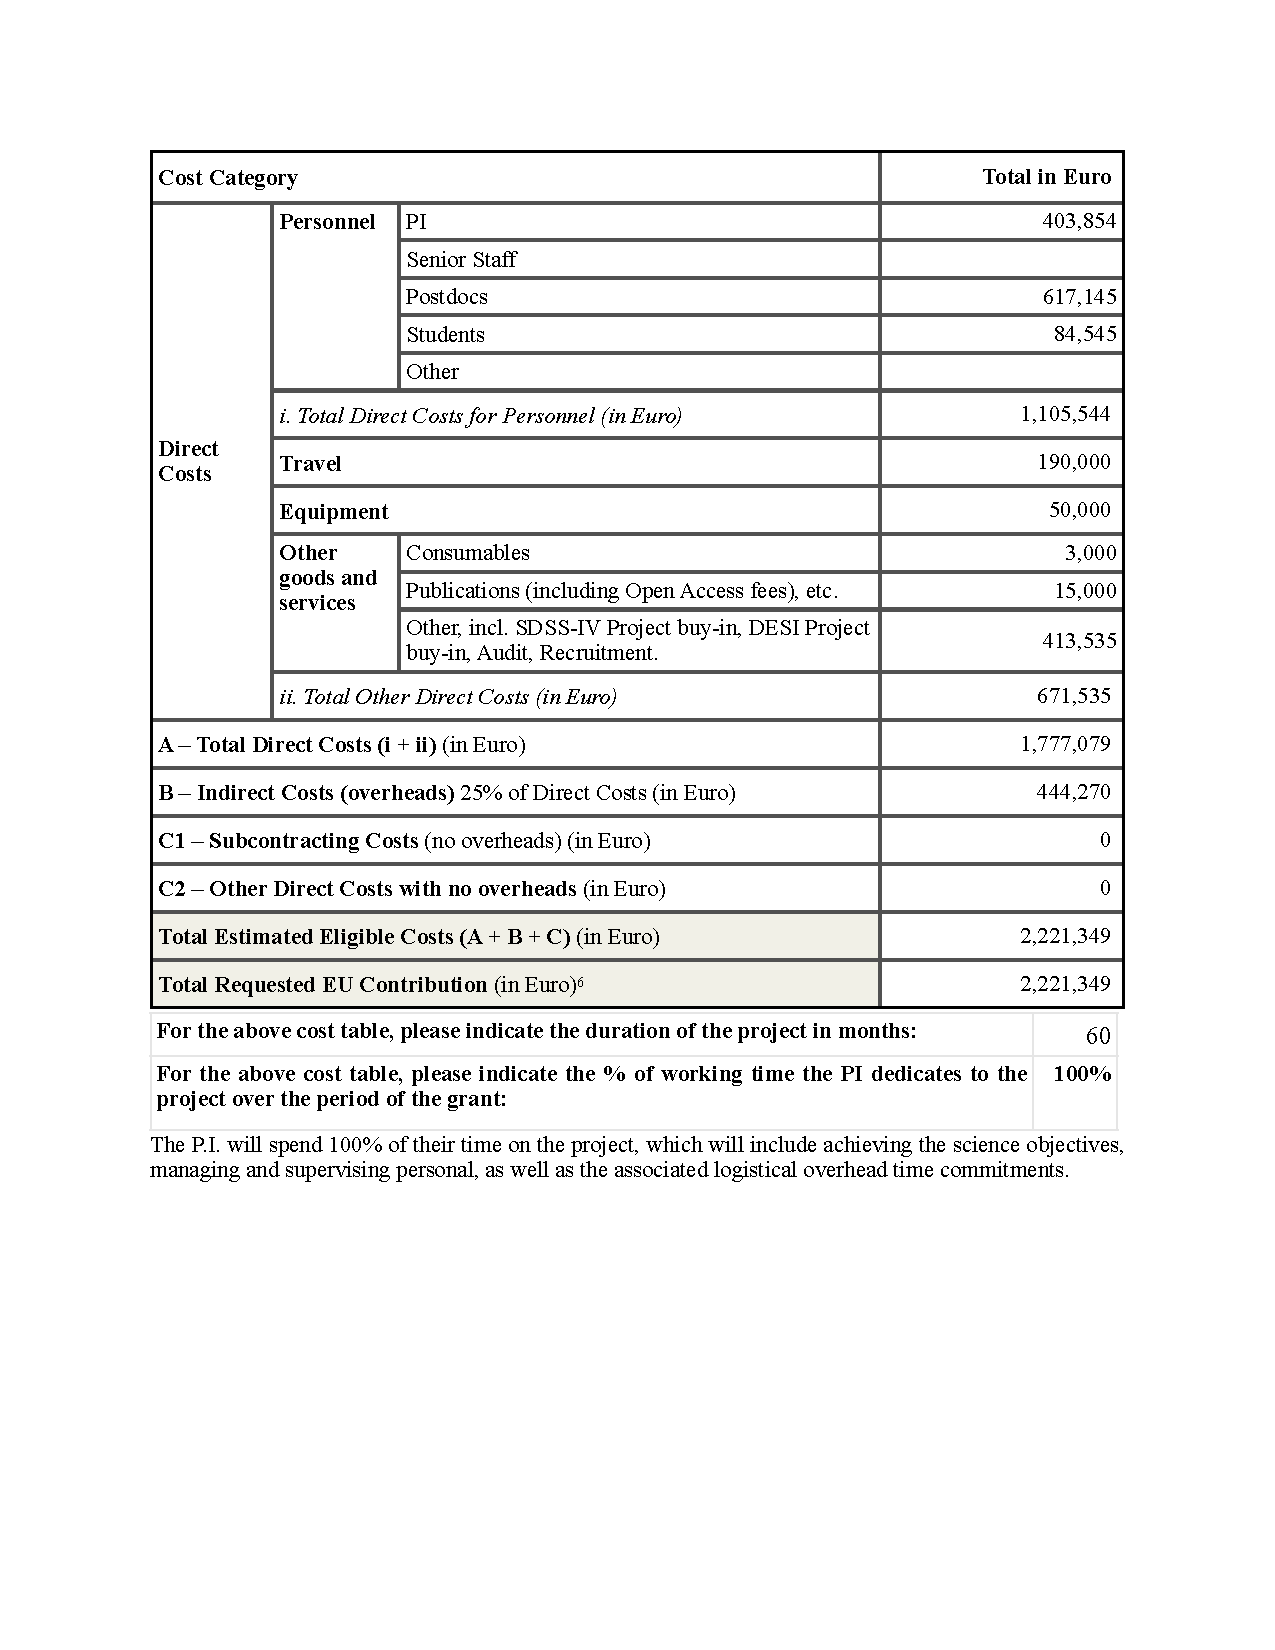
\includegraphics[width=16.6cm]
    {ResourcesSummary.pdf}
    \vspace{-10pt}
%    \caption{%\small            \footnotesize       % \scriptsize      % \tiny
%      {\it (Left:)} The optical and infrared light-curve for J110057; 
  %    Note the fall in the infrared, whereas there is a decrease, but 
    %  then recovery in the optical. 
     % {\it (Right:)} 
     % Three epochs of spectra for J110057. 
     % The spectacular downturn in the blue for the 2010 spectrum 
      %indicates a dramatic change in the accretion disk.
   % }
  \vspace{-16pt}
 \label{fig:J110057}
\end{center}
\end{figure}


\smallskip
\smallskip
\noindent
\textbf{\textsc{Team Compositon:}}
Our team will consist of the P.I, three postdoctoral research
associates (PDRAs), and 1 PhD student.  Two postdoctoral appointmenst
will be for three years each and one will be for a four year
appointment (a total of 10 FTE over 5 years).  The one PhD student
will have a four year appointment.  The ambitious nature of this
project requires a large team of both observational and theoretical
postdoctoral scholars and PhD students to complete the proposed
research.  The P.I. is not a current member of academic staff and
therefore has no responsibilities extending beyond research.  As such,
the P.I. is charged at 100\% and, if successful, will focus solely on
the aims of the project.  Again, this will be necessary to achieve all
our goals on the given schedule.

\smallskip \smallskip
\noindent \textbf{\textsc{Salaries:}} The primary expenditure of our
project corresponds to salaries in order support the large team
necessary for this project.  The P.I will be fully involved (project
management, scientific analysis, student supervision, postdoc
mentorship, proposal writing, communication with external
collaborations, and paper writing) and is covered at the 100\% level
over 5 years.  Salaries are determined according to the UoE salary
scale: \euro80.7k per FTE for the P.I, \euro61.3k per FTE for the
PDRAs and \euro21.1k per FTE for PhD students.  The total cost of
salaries over 5 years is {\bf \euro 1106k}.

\smallskip \smallskip
\noindent \textbf{\textsc{Travel:}} A major expense is in the form of
travel. I expect all group members to disseminate our results in
international conference but also to participate in external
collaboration meeting (at least one per year). Due to the nature and
timing of our proposal, it will almost certainly be critical for the
PDRAs to have extended (several week long) visits to the US and ESO
Chile. I have allocated thus allocated \euro10k/year for all members
of the group for travel. This level of commitment is necessary as has
been proved by the P.I.'s recent and continued involvement with the
e.g.  US-based surveys (and the benefit to his research
fellowship). The total travel budget is {\bf \euro190k.}

\smallskip
\smallskip
\noindent
\textbf{\textsc{Publications:}}
Our work will be published in international journals such as Nature,
Nature Astronomy, Science, Monthly Notices of the Royal Astronomical
Society and the Astrophysical Journal. I have allocated \euro3k/year for
the cost of publications. In addition, all papers will be on the arXiv
preprint server free of charge. The total publications budget is {\bf \euro15k.}

\smallskip
\smallskip
\noindent
\textbf{\textsc{Equipment \& Consumables:}}
I have allocated \euro10k/person for the initial purchase of a desktop
and laptop computer. Consumables are limited to \euro600/year (for the
purchase of back-up drives and other equipment). The total equipment
and consumables budget is {\bf \euro53k.}

\iffalse
\smallskip
\smallskip
\noindent
\textbf{\textsc{Visitors and Workshop:}}
I have also included a budget for inviting specialists to give
seminars and to discuss our results. The budget for inviting visitors
is \euro4k per year (corresponding to 2 to 4 visitors depending on if they
travel locally or internationally). In 2021 when all the team members
are present, I also plan to host a small invitation-only workshop (20
people total) on the topic of the quasar light-curve and spectal analysis. 
This will enable us bring together specialists from the field to advertise our
results but also to provide feedback on our work. For the workshop, I
have included a budget a \euro5k for the workshop organization (rent for
conference room, coffee breaks) and \euro10k to invite five invited
speakers and to help support travel costs for invited speakers
(\euro2k/person). The total budget for the workshop and visitors is {\bf \euro35k}.
\fi

\smallskip
\smallskip
\noindent
\textbf{\textsc{Access to Large Facilities:}}
We ask for additional funds that are availble to cover ``access to large facilities''. 
We request support for the ``buy-in'' to two of the new surveys,
SDSS-V and DESI. The costs here are \euro184.1k for
SDSS-V and \euro200.1k for DESI.  
%%
We specifically request access to these
funds as it gives our project access to telescopes and data in the
North and Southern Hemispheres (for complete coverage of the celestial
sphere) and delivers the crucial early spectroscopy that will be vital
to train, test and build our data science and machine learning codes
and algorithms.  We emphasise that the science return is `exponential'
(rather than `linearly') dependent on the breadth of data available
and heralds a brand new regime of ``several-survey'' or
``multi-mission'' astronomy. 
Buy-in allows the two observational PDRAs along with the PhD student 
to have data access rights here and 
 {\it would place the
P.I. and the University of Edinburgh as the only group and institute
in the world to be involved in SDSS-V, DESI, 4MOST, LSST and ESA {\it
Euclid} and JWST}.
The total budget for the access to large facilites is {\bf \euro384.2k}.

\smallskip
\smallskip
\noindent
Total budget before faciliites costs: \textbf{\underline{\euro this amount}}. \\
Total budget including faciliites costs: \textbf{\underline{\euro this amount+384.2k}}.\\

